% !TEX TS-program = pdflatexmk
\RequirePackage{atbegshi}
\documentclass[11pt,twoside]{article}

\usepackage{tikz}
\usetikzlibrary{positioning,shapes,arrows}

%%%%%%%%%%%%%%%%%%%%%%%%%%%
%
%  Font
%
%%%%%%%%%%%%%%%%%%%%%%%%%%%
\usepackage[sc]{mathpazo}
\linespread{1.05}         % Palatino needs more leading (space between lines)


%%%%%%%%%%%%%%%%%%%%%%%%%%%
%
%  Page Layout
%
%%%%%%%%%%%%%%%%%%%%%%%%%%%
\usepackage[margin=1in]{geometry} %changes margins
%\usepackage[parfill]{parskip} % begin paragraphs with an empty line not indent
\usepackage{multicol}


%%%%%%%%%%%%%%%%%%%%%%%%%%%
%
%  Page Header
%
%%%%%%%%%%%%%%%%%%%%%%%%%%%
\usepackage{fancyhdr}
\pagestyle{fancy}
\fancyhead{}
\fancyfoot{}
\renewcommand{\headrulewidth}{0pt}
\renewcommand{\footrulewidth}{0pt}
\fancyhead[LE,RO]{\thepage}   %page numbers

\fancyhead[CE]{\small CVEN 5313 FALL 2010}
\fancyhead[CO]{\small Problem Set 5}


%%%%%%%%%%%%%%%%%%%%%%%%%%%
%
%  Mathematics
%
%%%%%%%%%%%%%%%%%%%%%%%%%%%
\usepackage{amsmath,amssymb,amsthm,esint}
\usepackage{cancel}
\newcommand{\p}[2]{\frac{\partial#1}{\partial#2}}

% roman numerals
\makeatletter
\newcommand{\rmnum}[1]{\romannumeral #1}
\newcommand{\Rmnum}[1]{\expandafter\@slowromancap\romannumeral #1@}
\makeatother

\renewcommand{\d}{\partial}
%\newcommand{\vect}[1]{\underbar{#1}}
\newcommand{\vect}[1]{\vec{#1}}
\newcommand{\grad}{\nabla}
\newcommand{\tensor}[1]{\underline{\underline{#1}}}
\newcommand{\cross}{\times}
\newcommand{\curl}{\mbox{curl}}
\newcommand{\gradf}{\mbox{grad}}
\newcommand{\divf}{\mbox{div}}
\newcommand{\inline}[1]{\mbox{$#1$}}
\newcommand{\lint}{\ointctrclockwise}

\usepackage[pdftex,bookmarks,colorlinks,breaklinks]{hyperref}
\hypersetup{linkcolor=black,citecolor=black,filecolor=black,urlcolor=black}
\begin{document}


\thispagestyle{empty}
\noindent\textbf{Cameron Bracken}\\
CVEN 5313, Fall 2010\\
Problem Set 5


\begin{enumerate}

%%%%%%%%%%%%%%%%%%%%%%%%%%%%%%%%%%%%%%%%%%%%%
%
% Problem 1
%
%%%%%%%%%%%%%%%%%%%%%%%%%%%%%%%%%%%%%%%%%%%%%
\item 
\begin{enumerate}

%%%%%%%%%%%%%%%%%%%%%%%%%%%%%%%%%%%%%%%%%%%%%
%%%%%%%%%%%%%%%%%%%%%%%%%%%%%%%%%%%%%%%%%%%%%
\item In time $dt$ a differential element $dS$ expands or contracts at a rate $\vect{u}$ in the direction $\hat{n}$. So the change in volume of the element is

$$dV_{element}=\vect{u}\cdot\hat{n}\,dS\,dt.$$

Integrating (summing up) all the differential elements on the surface 

$$\iint_{S(t)}dV_{element}=\iint_{S(t)}\vect{u}\cdot\hat{n}\,dS\,dt$$
$$\frac{dV(t)}{dt}=\iint_{S(t)}\vect{u}\cdot\hat{n}\,dS$$

%%%%%%%%%%%%%%%%%%%%%%%%%%%%%%%%%%%%%%%%%%%%%
%%%%%%%%%%%%%%%%%%%%%%%%%%%%%%%%%%%%%%%%%%%%%
\item 
$$\frac{dV(t)}{dt} = \iiint_{\mathcal{R}(t)}\grad\cdot\vect{u}\,dV$$
From part (a)
$$\frac{dV(t)}{dt} = \iint_{S(t)}\vect{u}\cdot\hat{n}\,dS = \iint_{S(t)}\vect{u}\cdot\,d\vect{S}$$
Where $\hat{n}\,dS=d\vect{S}$. So by analogy to the divergence theorem ($\vect{u}=\tensor{T}$)
$$\frac{dV(t)}{dt} = \iiint_{\mathcal{R}(t)}\grad\cdot\vect{u}\,dV$$

\item $\grad\cdot\vect{u}$ can be interpreted as the expansion or contraction of a fluid volume due to the velocity field. 
\end{enumerate}

%%%%%%%%%%%%%%%%%%%%%%%%%%%%%%%%%%%%%%%%%%%%%
%
% Problem 2
%
%%%%%%%%%%%%%%%%%%%%%%%%%%%%%%%%%%%%%%%%%%%%%
\item 
\begin{enumerate}
\item[]

Consider a function $f(x_1,t)$ defined over a region $\mathcal{R}$.  The three dimensional Liebnitz formula is: 
\begin{equation}
\frac{d}{dt}\iiint_{R(t)}f(x_1,t)dV = \iiint_V \p{f}{t} dV + \iint_A n_k w_k f\: dA\label{lieb}
\end{equation}
Exmaining the first term on the left hand side, 
\begin{align}
\frac{d}{dt}\iiint_{R(t)}f(x_1,t)dV &= \frac{d}{dt}\iiint_{R(t)}f(x_1,t)dx_1dx_2dx_3\nonumber\\
                                    &= \frac{d}{dt}\int_{a(t)}^{b(t)}f(x_1,t)dx_1\iint_Adx_2dx_3\nonumber\\
                                    &= A\frac{d}{dt}\int_{a(t)}^{b(t)}f(x_1,t)dx_1\label{lhs}
\end{align}

Now examine the first term on the right hand side of \autoref{lieb}
\begin{align}
\iiint_V \p{f}{t} dV &= \iiint_V \p{f}{t} dx_1dx_2dx_3\nonumber\\
&=A\int_a^b \p{f}{t} dx_1\label{rhs1}
\end{align}

Next, examine the second term on the right hand side of \autoref{lieb}. Use a rectangular region with face areas $A_A=A_B=A$ (in the $x_2-x_3$ plane). Since the other faces have normal vectors orthoginal to the $x_1$ direction we don't need to consider them because $f$ is only a function of $x_1$ so 

$$
\iint_A n_k w_k f\: dA = \iint_{A_A} n_k w_k f\: dx_2\,dx_3 + \iint_{A_B} n_k w_k f\: dx_2\,dx_3 $$
For face $A$, $n_k$ points in the negative $x_1$ direction and $w_k$ is the rate of chage of the position of the face, $da/dt$. For face $B$, $n_k$ points in the positive $x_1$ direction and $w_k$ is the rate of chage of the position of the face, $db/dt$, so

\begin{align}
&= \iint_{A_A} (-1) \frac{da}{dt} f (a,t)\: dx_2\,dx_3 + \iint_{A_B} (1) \frac{db}{dt} f (b,t)\: dx_2\,dx_3 \nonumber\\
                       &=  - \frac{da}{dt} f (a,t)\iint_{A_A}\: dx_2\,dx_3 + \frac{db}{dt} f (b,t)\iint_{A_B}\: dx_2\,dx_3 \nonumber\\
                       & = \frac{db}{dt} f (b,t) A - \frac{da}{dt} f (a,t)A\label{rhs2}
\end{align}

Finally combine Equations \ref{lhs}, \ref{rhs1} and \ref{rhs2}

$$A\frac{d}{dt}\int_{a(t)}^{b(t)}f(x_1,t)dx_1 = A\int_a^b \p{f}{t} dx_1 + \frac{db}{dt} f (b,t) A - \frac{da}{dt} f (a,t)A$$

And divide by $A$

$$\frac{d}{dt}\int_{a(t)}^{b(t)}f(x_1,t)dx_1 = \int_a^b \p{f}{t} dx_1 + \frac{db}{dt} f (b,t)  - \frac{da}{dt} f (a,t).$$
\end{enumerate}

%%%%%%%%%%%%%%%%%%%%%%%%%%%%%%%%%%%%%%%%%%%%%
%
% Problem 3
%
%%%%%%%%%%%%%%%%%%%%%%%%%%%%%%%%%%%%%%%%%%%%%
\item 
\begin{enumerate}
\item $$\iiint_{\mathcal{R}}\grad\cdot\vect{u}\,dV = \iiint_{\mathcal{R}}0\,dV = 0$$

% Created by Eps2pgf 0.7.0 (build on 2008-08-24) on Wed Oct 27 03:01:26 MDT 2010
\begin{pgfpicture}
\pgfpathmoveto{\pgfqpoint{5.997cm}{14.005cm}}
\pgfpathlineto{\pgfqpoint{17.357cm}{14.005cm}}
\pgfpathlineto{\pgfqpoint{17.357cm}{23.424cm}}
\pgfpathlineto{\pgfqpoint{5.997cm}{23.424cm}}
\pgfpathclose
\pgfusepath{clip}
\pgfsetdash{}{0cm}
\pgfsetlinewidth{0.353mm}
\pgfsetmiterlimit{4.0}
\definecolor{eps2pgf_color}{cmyk}{0,0,0,1}\pgfsetstrokecolor{eps2pgf_color}\pgfsetfillcolor{eps2pgf_color}
\pgfpathmoveto{\pgfqpoint{13.502cm}{14.216cm}}
\pgfpathcurveto{\pgfqpoint{13.099cm}{15.304cm}}{\pgfqpoint{7.103cm}{18.06cm}}{\pgfqpoint{6.014cm}{17.657cm}}
\pgfusepath{stroke}
\pgfsetdash{}{0cm}
\pgfpathmoveto{\pgfqpoint{16.57cm}{18.694cm}}
\pgfpathcurveto{\pgfqpoint{16.167cm}{19.783cm}}{\pgfqpoint{10.171cm}{22.538cm}}{\pgfqpoint{9.082cm}{22.135cm}}
\pgfusepath{stroke}
\pgfsetdash{}{0cm}
\pgfpathmoveto{\pgfqpoint{6.014cm}{17.657cm}}
\pgfpathlineto{\pgfqpoint{9.082cm}{22.135cm}}
\pgfusepath{stroke}
\pgfsetdash{}{0cm}
\pgfpathmoveto{\pgfqpoint{13.502cm}{14.216cm}}
\pgfpathlineto{\pgfqpoint{16.57cm}{18.694cm}}
\pgfusepath{stroke}
\pgfsetdash{}{0cm}
\pgfpathmoveto{\pgfqpoint{11.459cm}{18.694cm}}
\pgfpathlineto{\pgfqpoint{12.518cm}{22.866cm}}
\pgfusepath{stroke}
\pgfpathmoveto{\pgfqpoint{12.57cm}{23.072cm}}
\pgfpathcurveto{\pgfqpoint{12.582cm}{22.966cm}}{\pgfqpoint{12.613cm}{22.83cm}}{\pgfqpoint{12.659cm}{22.739cm}}
\pgfpathlineto{\pgfqpoint{12.511cm}{22.839cm}}
\pgfpathlineto{\pgfqpoint{12.334cm}{22.821cm}}
\pgfpathcurveto{\pgfqpoint{12.418cm}{22.879cm}}{\pgfqpoint{12.51cm}{22.984cm}}{\pgfqpoint{12.57cm}{23.072cm}}
\pgfusepath{fill}
\pgfsetdash{}{0cm}
\pgfpathmoveto{\pgfqpoint{10.262cm}{14.041cm}}
\pgfpathlineto{\pgfqpoint{10.794cm}{16.136cm}}
\pgfusepath{stroke}
\pgfsetdash{{0.071cm}{0.071cm}}{0cm}
\pgfpathmoveto{\pgfqpoint{10.794cm}{16.136cm}}
\pgfpathlineto{\pgfqpoint{11.381cm}{18.447cm}}
\pgfusepath{stroke}
\pgfpathmoveto{\pgfqpoint{11.433cm}{18.653cm}}
\pgfpathcurveto{\pgfqpoint{11.445cm}{18.547cm}}{\pgfqpoint{11.476cm}{18.411cm}}{\pgfqpoint{11.522cm}{18.32cm}}
\pgfpathlineto{\pgfqpoint{11.374cm}{18.42cm}}
\pgfpathlineto{\pgfqpoint{11.196cm}{18.402cm}}
\pgfpathcurveto{\pgfqpoint{11.28cm}{18.461cm}}{\pgfqpoint{11.373cm}{18.565cm}}{\pgfqpoint{11.433cm}{18.653cm}}
\pgfusepath{fill}
\pgftext[x=13.959cm,y=22.101cm,rotate=0]{$\vect{u}\cdot d\vect{S}$ out}
\pgftext[x=9.343cm,y=15.517cm,rotate=0]{$\vect{u}\cdot d\vect{S}$ in}
\pgftext[x=7.325cm,y=18.759cm,rotate=0]{$dS$}
\begin{pgfscope}
\end{pgfscope}
\end{pgfpicture}

\item For an infinitesimal surface element $dS$ (shown above) if $\grad\cdot\vect{u}=0$ then the velocity flux in $\vect{u}\cdot\vect{S}$ will equal the velocity flux out so the total flux (in - out) will be zero.

\end{enumerate}

%%%%%%%%%%%%%%%%%%%%%%%%%%%%%%%%%%%%%%%%%%%%%
%
% Problem 4
%
%%%%%%%%%%%%%%%%%%%%%%%%%%%%%%%%%%%%%%%%%%%%%
\item
\begin{enumerate}
\item
$$\iint_A \hat{n}\cdot(\grad\cross\vect{u})\,dA = \iint_A\vect{\omega}\cdot\hat{n}\,dA$$
% Created by Eps2pgf 0.7.0 (build on 2008-08-24) on Wed Oct 27 03:12:05 MDT 2010
\begin{pgfpicture}
\pgfpathmoveto{\pgfqpoint{0cm}{0cm}}
\pgfpathlineto{\pgfqpoint{13.617cm}{0cm}}
\pgfpathlineto{\pgfqpoint{13.617cm}{5.115cm}}
\pgfpathlineto{\pgfqpoint{0cm}{5.115cm}}
\pgfpathclose
\pgfusepath{clip}
\pgfsetdash{}{0cm}
\pgfsetlinewidth{0.353mm}
\pgfsetmiterlimit{4.0}
\definecolor{eps2pgf_color}{cmyk}{0,0,0,1}\pgfsetstrokecolor{eps2pgf_color}\pgfsetfillcolor{eps2pgf_color}
\pgfpathmoveto{\pgfqpoint{1.535cm}{3.034cm}}
\pgfpathcurveto{\pgfqpoint{1.745cm}{3.006cm}}{\pgfqpoint{1.775cm}{2.814cm}}{\pgfqpoint{1.782cm}{2.646cm}}
\pgfpathmoveto{\pgfqpoint{1.27cm}{3.404cm}}
\pgfpathlineto{\pgfqpoint{1.711cm}{3.404cm}}
\pgfpathlineto{\pgfqpoint{1.711cm}{2.963cm}}
\pgfpathlineto{\pgfqpoint{1.27cm}{2.963cm}}
\pgfpathlineto{\pgfqpoint{1.27cm}{3.404cm}}
\pgfpathclose
\pgfpathmoveto{\pgfqpoint{0.758cm}{4.727cm}}
\pgfpathcurveto{\pgfqpoint{0.471cm}{4.619cm}}{\pgfqpoint{0.269cm}{3.918cm}}{\pgfqpoint{0.193cm}{3.669cm}}
\pgfpathcurveto{\pgfqpoint{0.028cm}{3.13cm}}{\pgfqpoint{0.035cm}{2.559cm}}{\pgfqpoint{0.034cm}{2.001cm}}
\pgfpathcurveto{\pgfqpoint{0.034cm}{1.4cm}}{\pgfqpoint{0.053cm}{0.401cm}}{\pgfqpoint{0.725cm}{0.108cm}}
\pgfpathcurveto{\pgfqpoint{1.079cm}{-0.046cm}}{\pgfqpoint{1.592cm}{0.052cm}}{\pgfqpoint{1.948cm}{0.128cm}}
\pgfpathcurveto{\pgfqpoint{2.409cm}{0.227cm}}{\pgfqpoint{2.879cm}{0.317cm}}{\pgfqpoint{3.335cm}{0.438cm}}
\pgfpathcurveto{\pgfqpoint{3.776cm}{0.554cm}}{\pgfqpoint{4.142cm}{0.715cm}}{\pgfqpoint{4.439cm}{1.076cm}}
\pgfpathcurveto{\pgfqpoint{4.566cm}{1.231cm}}{\pgfqpoint{4.726cm}{1.415cm}}{\pgfqpoint{4.728cm}{1.627cm}}
\pgfpathcurveto{\pgfqpoint{4.73cm}{1.776cm}}{\pgfqpoint{4.664cm}{1.786cm}}{\pgfqpoint{4.626cm}{1.913cm}}
\pgfpathcurveto{\pgfqpoint{4.566cm}{2.114cm}}{\pgfqpoint{4.624cm}{2.401cm}}{\pgfqpoint{4.622cm}{2.608cm}}
\pgfpathcurveto{\pgfqpoint{4.618cm}{3.134cm}}{\pgfqpoint{4.424cm}{3.687cm}}{\pgfqpoint{4.06cm}{4.083cm}}
\pgfpathcurveto{\pgfqpoint{3.601cm}{4.582cm}}{\pgfqpoint{2.838cm}{4.61cm}}{\pgfqpoint{2.256cm}{4.886cm}}
\pgfpathcurveto{\pgfqpoint{1.954cm}{5.03cm}}{\pgfqpoint{1.715cm}{5.201cm}}{\pgfqpoint{1.397cm}{4.97cm}}
\pgfpathcurveto{\pgfqpoint{1.263cm}{4.873cm}}{\pgfqpoint{1.248cm}{4.852cm}}{\pgfqpoint{1.076cm}{4.815cm}}
\pgfpathcurveto{\pgfqpoint{0.978cm}{4.795cm}}{\pgfqpoint{0.861cm}{4.762cm}}{\pgfqpoint{0.758cm}{4.727cm}}
\pgfusepath{stroke}
\pgftext[x=1.829cm,y=2.446cm,rotate=0]{$dS$}
\pgfsetdash{}{0cm}
\pgfpathmoveto{\pgfqpoint{9.084cm}{2.364cm}}
\pgfpathlineto{\pgfqpoint{7.038cm}{1.923cm}}
\pgfpathlineto{\pgfqpoint{6.342cm}{3.9cm}}
\pgfpathlineto{\pgfqpoint{8.361cm}{4.128cm}}
\pgfpathlineto{\pgfqpoint{9.084cm}{2.364cm}}
\pgfpathclose
\pgfusepath{stroke}
\pgftext[x=6.697cm,y=1.194cm,rotate=0]{$dS$}
\pgfsetdash{}{0cm}
\pgfpathmoveto{\pgfqpoint{7.713cm}{3.184cm}}
\pgfpathlineto{\pgfqpoint{8.237cm}{3.404cm}}
\pgfusepath{stroke}
\pgfpathmoveto{\pgfqpoint{8.3cm}{3.47cm}}
\pgfpathcurveto{\pgfqpoint{8.24cm}{3.464cm}}{\pgfqpoint{8.198cm}{3.464cm}}{\pgfqpoint{8.148cm}{3.463cm}}
\pgfpathlineto{\pgfqpoint{8.217cm}{3.299cm}}
\pgfpathcurveto{\pgfqpoint{8.229cm}{3.313cm}}{\pgfqpoint{8.281cm}{3.364cm}}{\pgfqpoint{8.328cm}{3.403cm}}
\pgfpathcurveto{\pgfqpoint{8.379cm}{3.444cm}}{\pgfqpoint{8.426cm}{3.478cm}}{\pgfqpoint{8.458cm}{3.497cm}}
\pgfpathcurveto{\pgfqpoint{8.422cm}{3.487cm}}{\pgfqpoint{8.365cm}{3.477cm}}{\pgfqpoint{8.3cm}{3.47cm}}
\pgfusepath{fill}
\pgfsetdash{}{0cm}
\pgfpathmoveto{\pgfqpoint{7.713cm}{3.184cm}}
\pgfpathlineto{\pgfqpoint{9.313cm}{1.041cm}}
\pgfusepath{stroke}
\pgfpathmoveto{\pgfqpoint{9.392cm}{0.996cm}}
\pgfpathcurveto{\pgfqpoint{9.371cm}{1.053cm}}{\pgfqpoint{9.362cm}{1.093cm}}{\pgfqpoint{9.349cm}{1.142cm}}
\pgfpathlineto{\pgfqpoint{9.206cm}{1.035cm}}
\pgfpathcurveto{\pgfqpoint{9.223cm}{1.027cm}}{\pgfqpoint{9.285cm}{0.988cm}}{\pgfqpoint{9.334cm}{0.952cm}}
\pgfpathcurveto{\pgfqpoint{9.386cm}{0.913cm}}{\pgfqpoint{9.431cm}{0.876cm}}{\pgfqpoint{9.456cm}{0.849cm}}
\pgfpathcurveto{\pgfqpoint{9.438cm}{0.881cm}}{\pgfqpoint{9.414cm}{0.934cm}}{\pgfqpoint{9.392cm}{0.996cm}}
\pgfusepath{fill}
\pgfsetdash{}{0cm}
\pgfpathmoveto{\pgfqpoint{7.713cm}{3.184cm}}
\pgfpathlineto{\pgfqpoint{9.084cm}{3.757cm}}
\pgfusepath{stroke}
\pgfpathmoveto{\pgfqpoint{9.147cm}{3.823cm}}
\pgfpathcurveto{\pgfqpoint{9.086cm}{3.816cm}}{\pgfqpoint{9.045cm}{3.817cm}}{\pgfqpoint{8.995cm}{3.816cm}}
\pgfpathlineto{\pgfqpoint{9.063cm}{3.652cm}}
\pgfpathcurveto{\pgfqpoint{9.076cm}{3.666cm}}{\pgfqpoint{9.128cm}{3.717cm}}{\pgfqpoint{9.175cm}{3.755cm}}
\pgfpathcurveto{\pgfqpoint{9.225cm}{3.797cm}}{\pgfqpoint{9.273cm}{3.831cm}}{\pgfqpoint{9.305cm}{3.849cm}}
\pgfpathcurveto{\pgfqpoint{9.269cm}{3.839cm}}{\pgfqpoint{9.212cm}{3.829cm}}{\pgfqpoint{9.147cm}{3.823cm}}
\pgfusepath{fill}
\pgftext[x=9.084cm,y=0.712cm,rotate=0]{$\vect{\omega}$}
\pgftext[x=9.089cm,y=4.207cm,rotate=0]{$\vect{\omega}\cdot\hat{n}$}

\pgftext[x=7.653cm,y=3.598cm,rotate=0]{$\hat{n}$}
\begin{pgfscope}
\end{pgfscope}
\end{pgfpicture}


\item If we slice the surface at an arbitratry location, we get two pieces $a$, $b$, with volumes $V_a$ and $V_b$ where $V_a+V_b=V$.  To find the total flux across the sliced faces, we need to integrate $\vect{\omega}d\vect{A}$ for both faces $A_b$, $A_b$. 

\begin{align*}
\iint_A\vect{\omega}d\vect{A} &= \iint_{A_a}\vect{\omega}d\vect{A}_a + \iint_{A_b}\vect{\omega}d\vect{A}_b\\
&=\lint_{C_a}\vect{u}\cdot d\vect{\ell}_{a} + \lint_{C_b}\vect{u}\cdot d\vect{\ell}_{b}
\end{align*}
By inspection the tangent vectors to both curves are equal and opposite, $d\vect{\ell}_{a} = -d\vect{\ell}_{b}$, and since $C_a$ and $C_b$ are the same curve 

$$\lint_{C_a}\vect{u}\cdot d\vect{\ell}_{a} - \lint_{C_b}\vect{u}\cdot d\vect{\ell}_{a} = 0 $$

So 

$$\iint_A\vect{\omega}d\vect{A} = 0 .$$

\item 
$$\iint \grad\cdot\vect{u}d\vect{A} = \iiint_{\mathcal{R}}\grad\cdot(\grad\cdot\vect{u})dV = \iiint_{\mathcal{R}}0dV = 0$$

Since $\grad\cdot(\grad\cdot\vect{u}) = \divf(\curl(\vect{u})) = 0$ from the previous problem set. 

\end{enumerate}


%%%%%%%%%%%%%%%%%%%%%%%%%%%%%%%%%%%%%%%%%%%%%
%
% Problem 5
%
%%%%%%%%%%%%%%%%%%%%%%%%%%%%%%%%%%%%%%%%%%%%%
\item 
\begin{enumerate}

%%%%%%%%%%%%%%%%%%%%%%%%%%%%%%%%%%%%%%%%%%%%%
%%%%%%%%%%%%%%%%%%%%%%%%%%%%%%%%%%%%%%%%%%%%%
\item 
$$\omega_3=\left[\p{u_2}{x_1}-\p{u_1}{x_2}\right]$$

For a differential element Stokes' theorem says

\begin{equation}
\vect{\omega}\cdot d\vect{A}=\vect{u}\cdot d\vect{\ell}\label{stokes}
\end{equation}

Consider the differential element below where the velocity field $\vect{u}$ is specified as $(u_1,u_2)$ at point $A$

%\begin{figure}[!h]
\begin{center}

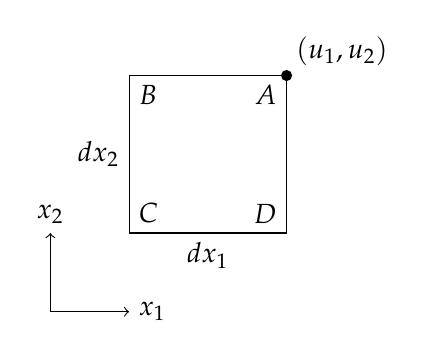
\begin{tikzpicture}[scale=2]
	\coordinate [label=below left:$A$] (A) at (1,1);
	\coordinate [label=below right:$B$] (B) at (0,1); 
	\coordinate [label=above right:$C$] (C) at (0,0);
	\coordinate [label=above left:$D$] (D) at (1,0);
	\draw (A) node[above right]{$(u_1,u_2)$}-- (B) -- node[left]{$dx_2$} (C) -- node[below]{$dx_1$} (D) -- cycle;

	\draw [->](-.5,-.5) -- (0,-.5) node[right] {$x_1$};
	\draw [->] (-.5,-.5) -- (-.5,0) node[above] {$x_2$};
	\node[fill,inner sep=.5mm,circle] at (A) {};

\end{tikzpicture}
\end{center}
%\end{figure}

If the element exists in the $x_1-x_2$ plane then the left hand side of \autoref{stokes} simplifies to $w_3dx_1dx_2$. Let $\vect{u}_{A\rightarrow B}$ be the velocity field along the line $AB$ for each line segment. Break down the right hand side of \autoref{stokes} for each of the edges of the element

\begin{equation}
\vect{u}\cdot d\vect{\ell} = 
\vect{u}_{A\rightarrow B}\cdot d\vect{\ell}_{A\rightarrow B} + 
\vect{u}_{B\rightarrow C}\cdot d\vect{\ell}_{B\rightarrow C} +
\vect{u}_{C\rightarrow D}\cdot d\vect{\ell}_{C\rightarrow D} +
\vect{u}_{D\rightarrow A}\cdot d\vect{\ell}_{D\rightarrow A}.
\label{line}
\end{equation}

The vector field along each of the segments can be written in terms of the specified point and the gradient (since the gradient is linear for a differential length).

\begin{align*}
\vect{u}_{A\rightarrow B} = (u_1, \bullet)\quad&\quad\vect{u}_{B\rightarrow C} = (\bullet, u_2-\p{u_2}{x_1}dx_1)\\
\vect{u}_{C\rightarrow D} = (u_1-\p{u_1}{x_2}dx_2, \bullet) \quad&\quad\vect{u}_{D\rightarrow A} = (\bullet,u_2)
\end{align*}

Where $\bullet$ is an actual component of the velocity field that does not need to be considered because it is perpendicular to the tangent vector $d\vect{\ell}$ for its respective segment. The tangent vectors are

\begin{align*}
d\vect{\ell}_{A\rightarrow B} = (-dx_1, 0)\quad&\quad d\vect{\ell}_{B\rightarrow C} = (0, -dx_2)\\
d\vect{\ell}_{C\rightarrow D} = (dx_1,0) \quad&\quad d\vect{\ell}_{D\rightarrow A} = (0,dx_2)
\end{align*}

Combining the terms in \autoref{line} and the left hand side of \autoref{stokes} gives

$$\omega_3dx_1dx_2 = -u_1dx_1 - u_2dx_2 + \p{u_2}{x_1}dx_1dx_2 +  u_1dx_1-\p{u_1}{x_2}dx_2dx_1 + u_2dx_2.$$

Canceling terms and dividing by $x_1x_2$ we end up with

$$\omega_3 =  \left[\p{u_2}{x_1}-\p{u_1}{x_2}\right].\qed$$
	
%%%%%%%%%%%%%%%%%%%%%%%%%%%%%%%%%%%%%%%%%%%%%
%%%%%%%%%%%%%%%%%%%%%%%%%%%%%%%%%%%%%%%%%%%%%
\item	

$$\omega_z=\frac{1}{r}\left[\p{}{r}(ru_\theta)\frac{u_r}{\theta}\right]$$


The logic is the same as in part (a). Consider a differential element in the $r-\theta$ plane

% Created by Eps2pgf 0.7.0 (build on 2008-08-24) on Wed Oct 27 02:41:00 MDT 2010
\begin{pgfpicture}
\pgfpathmoveto{\pgfqpoint{1.199cm}{5.891cm}}
\pgfpathlineto{\pgfqpoint{7.126cm}{5.891cm}}
\pgfpathlineto{\pgfqpoint{7.126cm}{12.982cm}}
\pgfpathlineto{\pgfqpoint{1.199cm}{12.982cm}}
\pgfpathclose
\pgfusepath{clip}
\begin{pgfscope}
\pgfpathmoveto{\pgfqpoint{2.534cm}{12.348cm}}
\pgfpathlineto{\pgfqpoint{6.061cm}{12.348cm}}
\pgfpathlineto{\pgfqpoint{6.061cm}{6.575cm}}
\pgfpathlineto{\pgfqpoint{2.534cm}{6.575cm}}
\pgfpathlineto{\pgfqpoint{2.534cm}{12.348cm}}
\pgfpathclose
\pgfusepath{clip}
\pgfsetdash{}{0cm}
\pgfsetlinewidth{0.353mm}
\pgfsetmiterlimit{4.0}
\definecolor{eps2pgf_color}{cmyk}{0,0,0,1}\pgfsetstrokecolor{eps2pgf_color}\pgfsetfillcolor{eps2pgf_color}
\pgfpathmoveto{\pgfqpoint{2.541cm}{12.331cm}}
\pgfpathcurveto{\pgfqpoint{3.751cm}{12.331cm}}{\pgfqpoint{4.952cm}{11.941cm}}{\pgfqpoint{5.931cm}{11.23cm}}
\pgfusepath{stroke}
\pgfsetdash{{0.071cm}{0.071cm}}{0cm}
\pgfpathmoveto{\pgfqpoint{5.247cm}{10.305cm}}
\pgfpathcurveto{\pgfqpoint{4.785cm}{10.64cm}}{\pgfqpoint{4.261cm}{10.887cm}}{\pgfqpoint{3.709cm}{11.032cm}}
\pgfpathcurveto{\pgfqpoint{3.329cm}{11.133cm}}{\pgfqpoint{2.935cm}{11.185cm}}{\pgfqpoint{2.541cm}{11.185cm}}
\pgfusepath{stroke}
\pgfsetdash{}{0cm}
\pgfpathmoveto{\pgfqpoint{2.541cm}{10.032cm}}
\pgfpathcurveto{\pgfqpoint{3.258cm}{10.032cm}}{\pgfqpoint{3.968cm}{9.802cm}}{\pgfqpoint{4.551cm}{9.387cm}}
\pgfusepath{stroke}
\pgfsetdash{{0.071cm}{0.071cm}}{0cm}
\pgfpathmoveto{\pgfqpoint{4.551cm}{9.387cm}}
\pgfpathlineto{\pgfqpoint{2.541cm}{6.579cm}}
\pgfusepath{stroke}
\pgfsetdash{}{0cm}
\pgfpathmoveto{\pgfqpoint{4.551cm}{9.387cm}}
\pgfpathlineto{\pgfqpoint{5.931cm}{11.23cm}}
\pgfusepath{stroke}
\pgfsetdash{{0.071cm}{0.071cm}}{0cm}
\pgfpathmoveto{\pgfqpoint{2.541cm}{10.032cm}}
\pgfpathlineto{\pgfqpoint{2.541cm}{6.579cm}}
\pgfusepath{stroke}
\pgfsetdash{}{0cm}
\pgfpathmoveto{\pgfqpoint{2.541cm}{10.032cm}}
\pgfpathlineto{\pgfqpoint{2.541cm}{12.331cm}}
\pgfusepath{stroke}
\pgfsetdash{{0.071cm}{0.071cm}}{0cm}
\pgfpathmoveto{\pgfqpoint{3.595cm}{9.865cm}}
\pgfpathlineto{\pgfqpoint{3.595cm}{9.865cm}}
\pgfusepath{stroke}
\pgfsetdash{{0.071cm}{0.071cm}}{0cm}
\pgfpathmoveto{\pgfqpoint{3.546cm}{9.88cm}}
\pgfpathlineto{\pgfqpoint{4.314cm}{12.05cm}}
\pgfusepath{stroke}
\pgfpathmoveto{\pgfqpoint{3.966cm}{10.965cm}}
\pgfpathcurveto{\pgfqpoint{3.966cm}{10.946cm}}{\pgfqpoint{3.95cm}{10.93cm}}{\pgfqpoint{3.93cm}{10.93cm}}
\pgfpathcurveto{\pgfqpoint{3.91cm}{10.93cm}}{\pgfqpoint{3.894cm}{10.946cm}}{\pgfqpoint{3.894cm}{10.965cm}}
\pgfpathcurveto{\pgfqpoint{3.894cm}{10.985cm}}{\pgfqpoint{3.91cm}{11.001cm}}{\pgfqpoint{3.93cm}{11.001cm}}
\pgfpathcurveto{\pgfqpoint{3.95cm}{11.001cm}}{\pgfqpoint{3.966cm}{10.985cm}}{\pgfqpoint{3.966cm}{10.965cm}}
\pgfusepath{fill}
\pgfsetdash{}{0cm}
\pgfpathmoveto{\pgfqpoint{3.966cm}{10.965cm}}
\pgfpathcurveto{\pgfqpoint{3.966cm}{10.946cm}}{\pgfqpoint{3.95cm}{10.93cm}}{\pgfqpoint{3.93cm}{10.93cm}}
\pgfpathcurveto{\pgfqpoint{3.91cm}{10.93cm}}{\pgfqpoint{3.894cm}{10.946cm}}{\pgfqpoint{3.894cm}{10.965cm}}
\pgfpathcurveto{\pgfqpoint{3.894cm}{10.985cm}}{\pgfqpoint{3.91cm}{11.001cm}}{\pgfqpoint{3.93cm}{11.001cm}}
\pgfpathcurveto{\pgfqpoint{3.95cm}{11.001cm}}{\pgfqpoint{3.966cm}{10.985cm}}{\pgfqpoint{3.966cm}{10.965cm}}
\pgfpathclose
\pgfusepath{stroke}
\pgfsetdash{}{0cm}
\pgfpathmoveto{\pgfqpoint{2.541cm}{7.659cm}}
\pgfpathcurveto{\pgfqpoint{2.769cm}{7.659cm}}{\pgfqpoint{2.994cm}{7.587cm}}{\pgfqpoint{3.179cm}{7.455cm}}
\pgfusepath{stroke}
\end{pgfscope}
\definecolor{eps2pgf_color}{cmyk}{0,0,0,1}\pgfsetstrokecolor{eps2pgf_color}\pgfsetfillcolor{eps2pgf_color}
\pgftext[x=2.928cm,y=7.788cm,rotate=0]{$d\theta$}
\pgftext[x=4.746cm,y=11.065cm,rotate=0]{$(u_r,u_\theta)$}
\begin{pgfscope}
\pgfpathmoveto{\pgfqpoint{2.534cm}{12.348cm}}
\pgfpathlineto{\pgfqpoint{6.061cm}{12.348cm}}
\pgfpathlineto{\pgfqpoint{6.061cm}{6.575cm}}
\pgfpathlineto{\pgfqpoint{2.534cm}{6.575cm}}
\pgfpathlineto{\pgfqpoint{2.534cm}{12.348cm}}
\pgfpathclose
\pgfusepath{clip}
\pgftext[x=4.62cm,y=12.064cm,rotate=0]{$(r+dr/2)d\theta$}
\end{pgfscope}
\pgftext[x=2.78cm,y=9.619cm,rotate=0]{$(r-dr/2)d\theta$}
\begin{pgfscope}
\pgfpathmoveto{\pgfqpoint{2.534cm}{12.348cm}}
\pgfpathlineto{\pgfqpoint{6.061cm}{12.348cm}}
\pgfpathlineto{\pgfqpoint{6.061cm}{6.575cm}}
\pgfpathlineto{\pgfqpoint{2.534cm}{6.575cm}}
\pgfpathlineto{\pgfqpoint{2.534cm}{12.348cm}}
\pgfpathclose
\pgfusepath{clip}
\pgfsetdash{}{0cm}
\pgfsetlinewidth{0.353mm}
\pgfsetmiterlimit{4.0}
\pgfpathmoveto{\pgfqpoint{4.551cm}{9.387cm}}
\pgfpathlineto{\pgfqpoint{4.677cm}{9.289cm}}
\pgfusepath{stroke}
\pgfsetdash{}{0cm}
\pgfpathmoveto{\pgfqpoint{5.931cm}{11.23cm}}
\pgfpathlineto{\pgfqpoint{6.057cm}{11.133cm}}
\pgfusepath{stroke}
\end{pgfscope}
\pgftext[x=5.429cm,y=10.25cm,rotate=0]{$dr$}
\begin{pgfscope}
\end{pgfscope}
\end{pgfpicture}


In this case $dA=rdrd\theta$ so we can rewrite the left hand side of \autoref{stokes} as $\omega_zrdrd\theta$.  Here we specify the falue of the velocity field at center point of the element so 

\begin{align*}
\vect{u}_{A\rightarrow B} = \left(u_r-\p{u_r}{\theta}\frac{d\theta}{2}, \bullet\right)\quad&\quad\vect{u}_{B\rightarrow C} = \left(\bullet, u_\theta+\p{u_\theta}{r}\frac{dr}{2}\right)\\
\vect{u}_{C\rightarrow D} = \left(u_r+\p{u_r}{\theta}\frac{d\theta}{2}, \bullet\right) \quad&\quad\vect{u}_{D\rightarrow A} = \left(\bullet,u_\theta-\p{u_\theta}{r}\frac{dr}{2}\right)
\end{align*}

and the tangent vectors are

\begin{align*}
d\vect{\ell}_{A\rightarrow B} = (dr, 0)\quad&\quad d\vect{\ell}_{B\rightarrow C} = (0, (r+dr/2)d\theta)\\
d\vect{\ell}_{C\rightarrow D} = (-dr,0) \quad&\quad d\vect{\ell}_{D\rightarrow A} = (0,-(r-dr/2)d\theta)
\end{align*}

Combining the terms in \autoref{line} and multiplying out the terms 

\begin{align*}
\omega_zrdrd\theta &= 
u_rdr-\p{u_r}{\theta}\frac{d\theta}{2}dr+
ru_\theta d\theta+
\p{u_\theta}{r}\frac{dr}{2}\frac{dr}{2}d\theta+
r\p{u_\theta}{r}\frac{dr}{2}d\theta+
u_\theta\frac{dr}{2}d\theta \\
& - u_rdr
-\p{u_r}{\theta}\frac{d\theta}{2}dr
-ru_\theta d\theta
-\p{u_\theta}{r}\frac{dr}{2}\frac{dr}{2} d\theta
+ r\p{u_\theta}{r}\frac{dr}{2}\p{u_r}{\theta}
+u_\theta\frac{dr}{2}d\theta \\
&= -\p{u_r}{\theta}d\theta dr + rdrd\theta\p{u_\theta}{d} + u_\theta drd\theta\\
\omega_z & = -\frac{1}{r}\p{u_r}{\theta} + \p{u_\theta}{d} + \frac{u_\theta}{r}\\
         & = \frac{1}{r}\left[ r\p{u_\theta}{r} + u_\theta\p{r}{r} - \p{u_r}{\theta}\right]\\
         & \mbox{By the reverse chain rule}\\
\omega_z & = \frac{1}{r}\left[ \p{}{r}(r u_\theta) - \p{u_r}{\theta}\right]\qed
\end{align*}

\end{enumerate}



\end{enumerate}






\end{document}
